\documentclass{article}
\usepackage[T1]{fontenc}
\usepackage{lmodern}
\usepackage{graphicx}
\usepackage{amsmath,amssymb}
\usepackage[a4paper,margin=2cm]{geometry}
\usepackage[absolute,overlay]{textpos}
\setlength{\TPHorizModule}{1mm}
\setlength{\TPVertModule}{1mm}
\usepackage[indonesian]{babel}
\usepackage{hyperref}
\setlength{\emergencystretch}{2em}
% unit: Halaman 12

\begin{document}

% === Halaman 12 (llm) ===

\vspace{163.35mm}

Round key 0 \vspace{5mm} putaran awal \vspace{5mm} $Nr - 1$ putaran \vspace{5mm} Round key $Nr - 1$ \vspace{5mm} putaran akhir

% deskripsi: Diagram alir proses enkripsi AES (Advanced Encryption Standard) yang menunjukkan tahapan State, AddRoundKey, SubBytes, ShiftRows, MixColumns, dan penggunaan Round Key dari putaran awal hingga putaran akhir.
% bbox normalisasi: [0.2500, 0.3300, 0.5500, 0.8800]
\begin{textblock*}{63.00mm}(52.50mm,98.01mm)
\noindent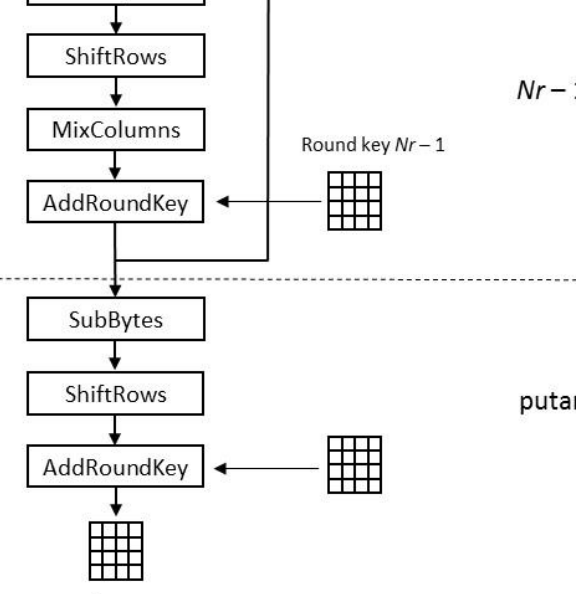
\includegraphics[width=63.00mm,height=163.35mm]{../../images/llm/page_012_img_01.png}%
\end{textblock*}

\end{document}
